\begin{figure}[htbp]
    \section*{ FGD1}
    \centering
    \begin{subfigure}[b]{0.95\textwidth}
    \centering
    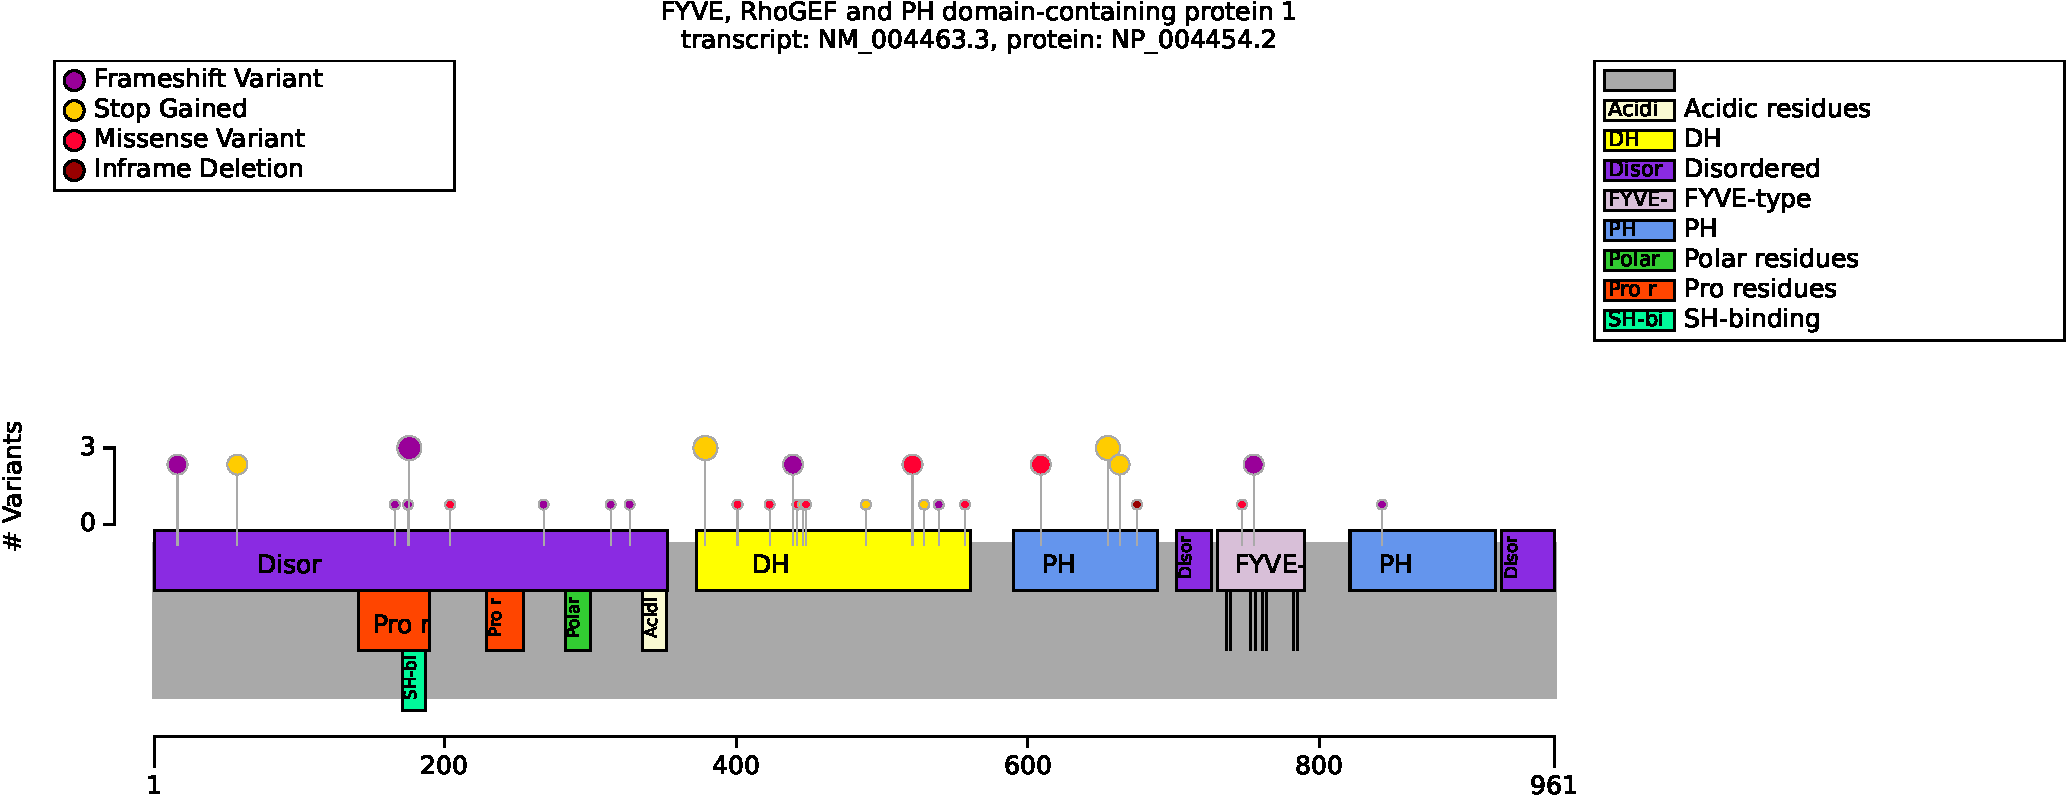
\includegraphics[width=\textwidth]{ img/FGD1_protein_diagram.pdf} 
    \captionsetup{justification=raggedright,singlelinecheck=false}
    \caption{Distribution of variants in FGD1}
    \end{subfigure}
    
    \vspace{2em}
    
    \begin{subfigure}[b]{0.95\textwidth}
    \centering
    \resizebox{\textwidth}{!}{
    \begin{tabular}{llllrr}
    \toprule
    HPO term & Missense & Other & p-value & adj. p-value\\
    \midrule
    Broad foot [HP:0001769] & 1/7 (14\%) & 14/15 (93\%) & $6.22\times 10^{-4}$ & 0.032\\
    \bottomrule
    \end{tabular}
    }
    \captionsetup{justification=raggedright,singlelinecheck=false}
    \caption{         Fisher Exact Test performed to compare HPO annotation frequency with respect to Missense and Other. Total of
            52 tests were performed. }
    \end{subfigure}
    \vspace{2em}
    \begin{subfigure}[b]{0.95\textwidth}
    \centering
    \resizebox{\textwidth}{!}{
    \begin{tabular}{llllrr}
    \toprule
    Genotype (A) & Genotype (B) & total tests performed & significant results\\
    \midrule
    DH domain & Other & 52 & 0\\
    \bottomrule
    \end{tabular}
    }
    \captionsetup{justification=raggedright,singlelinecheck=false}
    \caption{             Fisher Exact Test performed to compare HPO annotation frequency with respect to genotypes. }
    \end{subfigure}
    
    \vspace{2em}
    
    \caption{ The cohort comprised 48 individuals (0 females, 48 males). A total of 73 HPO terms were used to annotate the cohort. Disease diagnosis: Aarskog-Scott syndrome (OMIM:305400). Li et al (2024) identified a number of correlations including a lower frequency of Deformity of foot	
    (8/20) with missense than with "drastic" variants (29/41); p=0.03. Multiple testing correction was not performed \cite{PMID_38411716,PMID_33762894}.  A total of 35 unique variant alleles were found in \textit{FGD1} (transcript: \texttt{NM\_004463.3}, protein id: \texttt{NP\_004454.2}).}
    \end{figure}
    